\chapter{Method}
\label{chapter:method}

In this chapter I will describe two approaches to partial persistence. I will
analyse the asymptotic time and space complexities related to creating new
versions to the data structure and to retrieving an element in a desired
existing version.

\section{Background}

Tsotras and Kangelaris \cite{Tsotras1995237} define as the database state $s(t)$
the collection of objects that exist at time $t$ in the real-world system
modeled by the database. The ability to access $s(t)$ is here referred to as
``temporal access'', and is essentially the same as partial persistence in that
it allows read-only access to all versions and read/write access only to the
newest version. I will define the metric by which the approaches are measured as
the cost of producing $s(t)$ and navigating to an element within it.

I will analyse the following two approaches to obtaining partial persistence:
\begin{description}

  \item[Node copying] which requires structural extensions of the underlying
  data structure in order to store modification records and other necessary
  information within the nodes of the data structure; and

  \item[Rollback] which requires functional extensions of the underlying data
  structure in order to record the necessary information about the context in
  which an operation is carried out in order to be able to reproduce or revert
  it at a later time.

\end{description}

\section{The Node Copying method}
The purpose of the Node Copying method is to enable partial persistence in a
node-based data structure with bounded in-degree $p$ with an amortized constant
factor overhead on space and time complexity and providing transparent
navigation of the data structure.

Node Copying is a method described in \cite{Driscoll198986} by which a data
structure may be made partially persistent through the systematic expansion of
the node structure. An auxillary data structure maintaining entry points into
the data structure, such as which node is the head of a linked list, is also
introduced. These two modifications of the data structure enable queries to be
made with $O(1)$ factor amortized overhead and $O(1)$ factor space per change,
given that the original data structure has a bounded in-degree. In the
following, I will describe in detail the general procedure as well as giving the
concrete example of the linked list.

\subsection{Node structure expansion}
\label{subsec:node-structure-expansion}
In the Node Copying method, the node structure is expanded by adding two arrays;
one for ``modifications'' and one for ``back pointers''.

\paragraph{Persisting fields.}

The modifications array records changes made to any of the fields of the node,
including non-pointer fields, since the time when node was created --- the
original field values from the time of construction remain unchanged. A
modification record consist of a version number, a field identifier and a value.
When a fields is to be modified, a record is inserted in an empty slot of the
array.


To find the value of a field at a given version $v$, the modifications array is
looked through, and the most recent change before or at $v$ is returned. If no
modification is found, the original field value is returned.

In the Fat Node method described in \cite{Driscoll198986}, there is no upper
bound on the size of the modifications array. Therefore, the worst-case time to
retrieve a field value is linearly proportional with the number of
modifications.

\paragraph{Limited node size.}

To get constant factor amortized overhead for field access, the size of the
modifications array is bounded to the in-degree bound $p$. The time to retrieve
the field value is then at most $c \cdot p + k = O(1)$ where $c$ is the time it
takes to read each modification record and field identifiers and version
numbers, and $k$ is the time it takes to read the original field if neccessary.

If the modifications array is already occupied with previous changes when a new
change is required, a copy $n'$ of the original node $n$ is made. The fields of
$n'$ are set to the most recent versions of the fields in $n$, except that the
field which was to be changed is instead set to the required value. Note that
the modifications array of $n'$ is empty.

But if any nodes were -- in the most recent version -- pointing to $n$ prior to
the change, they will need to be updated to point to $n'$. To be able to know
which nodes were pointing to $n$, a ``back pointers'' array is maintained. Its
size must of course be equal to the in-degree bound $p$ to be able to contain
pointers to all nodes pointing to $n$. Whenever a pointer field in a node $y$ is
updated to point to another node $x$ (either when $y$ is constructed or when the
field is modified as described above), the corresponding back pointer in $x$ is
updated to point to $y$.

\paragraph{Cascading effects.}

When $n'$ is created, the back pointers of $n$ are followed, and each of the
nodes which pointed to $n$ will have a modification added referring to the
relevant field, and pointing to $n'$. But if the modifications array is already
full in one of these nodes, a copy of \emph{that} node will need to be made as
described above. This cascading effect can repeat.

For example, when an element $y$ is inserted at the head of a singly linked
list, its \textsc{next} pointer will point to the element $x$ which used to be
the head of the list. The ``\textsc{next}-back'' pointer in $x$ is then set to
point to $y$. If the modifications array of $x$ gets full and a copy $x'$ needs
to be made to allow a new modification, the ``\textsc{next}-back'' pointer is
followed to make a modification record in $y$ that in the new version, it should
point to $x'$ instead of $x$. But if a modification was already made to $y$,
e.g. its data field was updated, it will itself need to be copied according to
the same scheme --- i.e. there may be a cascading effect. In this example, where
$y$ was the head of the list, its copy $y'$ should be indicated as the new head
in the new version in the auxillary data structure.

\paragraph{Amortized constant factor overhead.}
To prove that -- even with cascading effects -- there is still a constant factor
amortized overhead per field change, we shall employ the potential technique.

The intuition is that for every time we copy a node $n$, the copy $n'$ will have
an empty modifications array, and thus it will take $p$ modifications to $n'$
before a new copy must be made. A node of which a copy has already been made
cannot be the target of yet another modification, and thus the available cheap
modifications to $n'$ account for the time spent on creating $n'$.

The following proof outline is based on the proof made in the original paper
\cite{Driscoll198986}, but a notable difference here is the absence of a copy
pointer, and the specification that the modifications are stored in a fixed-size
array.

We define a \emph{live node} as a node which can be reached in the most recent
version of the data structure, and a \emph{full} live node as a live node with a
full modifications array. Let the potential function $\Phi(v)$ be the number of
full live nodes at version $v$. Then the potential at the initial version
$\Phi(0)$ is zero, and since there cannot be a negative number of full live
nodes, the potential is always greater than or equal to zero.

The \emph{actual cost} of an update to a full live node which causes a total of
$k$ copies to be made (both due to the node itself being copied and due to any
cascading effects) is $O(k) + O(1)$ since each copy costs $O(1)$ both in space
and time, and modifying a field costs $O(1)$. For each of the copies created,
the original node is no longer live (since nodes pointing to it are updated to
point to the copy), and the modifications array of the copy is empty. Thus, each
copy decreases the potential by 1, and the \emph{total change in potential}
$\Delta\Phi$ is $O(-k)$ plus $O(1)$ in case the last update made via a back
pointer fills the modifications array of that node. Therefore, the amortized
time and space cost for the entire update operation is $O(k) + O(1) + (O(-k) +
O(1)) = O(1)$.

\section{The Rollback method}
Rollback is an approach to partial persistence based on the techniques described
in \cite{Tsotras1995237}, namely the combination of the na\"ive ``copy'' and
``log'' methods.

\subsection{The na\"ive approaches}
The ``copy'' approach makes a full copy of every version of the data structure
and makes it available by direct indexing to achieve $O(1)$ access overhead
factor. Creating each copy becomes more expensive in time and space the more
elements are inserted. In the worst case, when only insertions and no deletions
or modifications are made, the cost of creating $n$ versions is
$O\left(n^2\right)$.

The ``log'' approach conserves space by recording for each change made to the
data structure just enough information necessary to undo or redo it, thus giving
a space overhead factor per operation of $O(1)$. A ``current'' version
$v_{current}$ of the data structure is maintained. Given $v_{current}$, the
version $v_x$ can be produced by undoing or redoing all the changes between
$v_{current}$ and $v_x$ depending on which is the oldest. As the number of
versions $n$ increases, accessing a specific version becomes potentially more
costly. In the worst case, the overhead factor is $O(n)$ when $v_{current}$ is
$v_0$ and $v_x$ is $v_n$, or opposite.

\subsection{The hybrid approach}
\label{subsec:the-hybrid-approach}
An obvious hybrid of the two na\"ive approaches is to keep the records of each
operation like in the ``log'' approach, and storing a full copy like in the
``copy'' approach only once every $d$ versions. To access version $v_x$, the
nearest version to $v_x$ of which there exists a full copy, $v_s$, is retrieved
and a mutable copy of the data structure at that version is made. Then, using
the log of the versions from $v_s$ to $v_x$, the data structure corresponding to
$v_x$ is produced and returned.

In the rest of this document, the term Rollback refers to the hybrid approach.

To reach the full copy nearest to version number $v$, the following expression
is used:
$$ \left\lfloor \frac{v + \frac{d}{2}}{d} \right\rfloor $$ With this indexing
expression, full copies will be selected for all operations which are within
$\pm \frac{d}{2}$ versions.

Naturally, $d$ is a user parameter. If there are $n$ versions, there will be
$\left\lfloor \frac{n}{d} \right\rfloor$ full copies, and the maximum number of
operations to reach a specific version is then $O(k+\frac{d}{2})$, where $k$ is
the time required to retrieve the full copy. It is now easy to see that the
greater $d$ is, the fewer full copies will be made, and thus the space cost is
reduced accordingly. Likewise, the distance to the version in the middle between
two full copies increases with $d$, inducing a higher cost for producing that
version.

As an alternative to making a mutable copy of a full copy when a nearby version
is requested, one could instead allow the full copies to be mutable and moved
within $\pm\frac{d}{2}$ of their original location. This will increase the
maximum number of operations between a full copy and the desired version to $d$,
but will reduce greatly the time cost of making a working copy of the full copy.
If the full copies are originially uniformly distributed, direct lookup is still
possible, but it is then needed for each full copy to annotate which version it
represents. If $d$ is constant, this approach allows constant time access to any
version of the data structure.

For large enough data sets, physical memory limits may restrict the ability to
make new full copies. A way to defer this is to increase $d$ by a factor $c$
when near the limit and discard all but every $c$ full copy that exists. This
will free some memory for creating new full copies, but will increase the
distance between them to $d' = c \cdot d$. Therefore, the claim no longer holds
that the time to access any version of the data structure is constant. Also, the
time spent previously on creating the full copies which are now discarded is no
longer valuable.

The time required to make a changing operation to the latest version equals the
time required to produce $v_{latest}$, plus the time required to carry it out
using the underlying data structure, plus the time required to adding an
operation record to the log. Carrying out the operation depends on the operation
in question, but recording the operation in the log potentially requires extra
information, e.g. a \textsc{remove} operation needs to store information in the
log allowing the reproduction of the removed element. Thus, the time complexity
depends both on the operation in question and on the inverse operation, which
may have different time complexity bounds.

It is obvious that with a doubly linked list, the overhead factor for making a
change to the latest version is $O(1)$.

On the other hand, creating the full copy becomes more expensive the more
elements are inserted in the preceeding versions. Thus it is intuitively not
possible to show $O(1)$ factor amortized time overhead for a sequence of
\textsc{insert} operations long enough to cause a full copy to be made.

\subsection{Operations sequence optimization}
For certain underlying data structures, it may prove feasible to pre-process the
sequence of operations between a full copy $v_s$ and the requested version $v_x$
in order to reduce the actual work necessary to reach $v_x$.

Two different types of pre-processing to reduce work when dealing with a linked
list are presented here: Eliminating superfluous operations and reordering
operations. It is worth noting that both of these require knowledge of the
underlying data structure, and thus require more programming time to implement.

\subsubsection{Eliminating operations}
The sequence of operations between $v_s$ and $v_x$ may contain some operations
which will not need to be explicitly applied. The cases are, in the context of a
linked list:

\begin{enumerate}
  \item An \textsc{insert} operation followed by a \textsc{remove} operation at
  the same effective index --- both can be removed from the sequence since they
  cancel each other out.
  \label{item:elop-insert-remove}

  \item An \textsc{insert} or a \textsc{modify} operation followed by a
  \textsc{modify} operation at the same effective index --- the former can have
  its associated data value changed to that of the latter, and the latter can be
  removed from the sequence.
  \label{item:elop-insert-modify}

  \item A \textsc{modify} operation followed by zero or more \textsc{modify}
  operations and a \textsc{remove} operation at the same effective index --- the
  former can be removed from the sequence.
  \label{item:elop-modify-remove}
\end{enumerate}

Cases \ref{item:elop-insert-remove} and \ref{item:elop-insert-modify} may of
course be combined in the sequence of one \textsc{insert} operation, one or more
\textsc{modify} operations and finally a \textsc{remove} operataion.

\paragraph{Algorithm.}
Pseudo code for an algorithm handling those cases is found in Algorithm
\ref{alg:eliminate-ops}.

\begin{algorithm}[p]
  \caption{An algorithm for eliminating superfluous operations}
  \label{alg:eliminate-ops}
  \begin{algorithmic}[5]
    \Procedure{EliminateSuperfluousOps}{sequence of operations $S$}
      \For {each operation $o_i \in S$, from last to first}
        \If {\textsc{type}($o_i$) $\in \left\{\textsc{insert},\textsc{modify}\right\}$}
        \State $c\gets\textsc{index}(o_i)$
          \For {each operation $o_j \in \left\{S|j>i\right\}$}
            \Switch {$\textsc{type}(o_j)$}
              \Case{\textsc{insert}}
                \If {$\textsc{index}(o_j) \le c$}
                  \State $c \gets c+1$
                \EndIf
              \EndCase
              \Case{\textsc{modify}}
                \If {$\textsc{index}(o_j) = c$}
                  \State $\textsc{data}(o_i) \gets \textsc{data}(o_j)$
                  \State remove $o_j$ from $S$
                \EndIf
              \EndCase
              \Case{\textsc{remove}}
                \If {$\textsc{index}(o_j) < c$}
                  \State $c \gets c-1$
                \ElsIf {$\textsc{index}(o_j) = c$}
                  \Switch {$\textsc{type}(o_i)$}
                    \Case {\textsc{insert}}
                      \State $c \gets \textsc{index}(o_i)$
                      \For {each operation $o_k \in \left\{S|i<k<j\right\}$}
                        \If {$\textsc{index}(o_k) > c$}
                          \State $\textsc{index}(o_k) \gets \textsc{index}(o_k) - 1$
                        \Else
                          \Switch {\textsc{type}($o_k$)}
                            \Case {\textsc{insert}}
                              \If {$\textsc{index}(o_k) \le c$}
                                \State $c \gets c+1$
                              \EndIf
                            \EndCase
                            \Case {\textsc{remove}}
                              \If {$\textsc{index}(o_k) < c$}
                                \State $c \gets c-1$
                              \EndIf
                            \EndCase
                          \EndSwitch
                        \EndIf
                      \EndFor
                      \State remove $o_j$ from $S$
                      \State remove $o_i$ from $S$
                    \EndCase
                    \Case {\textsc{modify}}
                      \State remove $o_i$ from $S$
                    \EndCase
                  \EndSwitch
                \EndIf
              \EndCase
            \EndSwitch
          \EndFor
        \EndIf
      \EndFor
    \EndProcedure
  \end{algorithmic}
\end{algorithm}
 
The general idea is to identify cases \ref{item:elop-insert-remove},
\ref{item:elop-insert-modify} and \ref{item:elop-modify-remove} and make the
necessary maintenance before removing the relevant operations.

It iterates through the sequence backwards, i.e. from the last operation to the
first. If an \textsc{insert} or a \textsc{modify} operation $o_i$ is found, it
starts looking forwards for a matching \textsc{modify} or \textsc{remove}
operation. This is done by iterating through the proceeding operations while
keeping track of which index $c$ of the inserted or modified element would have
after each of the proceeding operations; if a proceeding operation $o_j$ inserts
or removes an element to the left of the originally inserted or modified
element, then the index would be shifted to the right or to the left,
respectively.

\newcommand{\specialcell}[2][c]{%
  \begin{tabular}[#1]{@{}l@{}}#2\end{tabular}}

If $o_j$ removes or modifies the element at index $c$, the type of $o_i$
determines what happens next. Table \ref{tab:oioj} shows which action is taken
depending on the types of $o_i$ and $o_j$.

\begin{table}[!ht]
  \center
  \begin{tabular}{|l|l|l|}\hline
    \diagbox{$o_i$\ \ }{$o_j$}&
    \textsc{modify} & \textsc{remove}\\
    \hline
    \textsc{insert} & update $o_i$ data, remove $o_j$ & \specialcell[t]{compensate between $o_i$ and $o_j$, \\ then remove both}\\
    \hline
    \textsc{modify} & update $o_i$ data, remove $o_j$ & remove $o_i$\\
    \hline
  \end{tabular}
  \caption{The table shows which action is taken depending on the types of $o_i$ and $o_j$.}
  \label{tab:oioj}
\end{table}

The compensation referred to in the case when $o_i$ is an \textsc{insert}
operation and $o_j$ is a \textsc{remove} operation works as follows:

\begin{itemize}

  \item Like in the iteration of the operations proceeding $o_i$, the index $c$
  of the inserted element is maintained while the operations between $o_i$ and
  $o_j$ (both exclusive) are iterated first to last.

  \item Since no operation prior to $o_j$ matches $o_i$, it is safe to assume
  that all operations between them have either greater or smaller indices than
  $c$. If an operation $o_k$ between $o_i$ and $o_j$ works on a smaller index,
  it will compensate the maintained index $c$ by -1 or +1. If $o_k$ works on a
  greater index, $o_k$ will itself have the index it works on reduced by 1,
  since its original index depended on the element of $o_i$ being inserted
  before it.

  \item When all operations between $o_i$ and $o_j$ have been examined thusly,
  $o_j$ and $o_i$ are removed from the sequence and the backwards iteration is
  resumed.

\end{itemize}

When the backwards iteration is finished examining the first operation in the
sequence, the algorithm terminates and the sequence now contains no operations
matching cases \ref{item:elop-insert-remove}, \ref{item:elop-insert-modify} or
\ref{item:elop-modify-remove}.

The space cost of the algorithm is in the order of the sequence size, i.e.
$O(1)$, since it works directly on the sequence. In the worst case, when all $n$
operations are \textsc{insert} or \textsc{modify} operations, the time cost is
$O\left(n^2\right)$, since with every \textsc{insert} operation, all the
proceeding operations are examined when a matching \textsc{remove} operation is
not found.

\subsubsection{Reordering operations}

Applying each operation in the sequence separately is potentially a time
expensive approach. Consider the case when each operation inserts an element at
the end of a linked list; the total cost for $n$ insertions on a list of length
$l$ would be $O\left(\left(l+n\right)^2\right)$ if every operation application
begins by iterating from the head of the list to the index of insertion.

It would indeed be more efficient to make the insertions in one straight
iteration of the linked list, which would cost $O(l+n)$; $l$ for reaching the
end of the list, $n$ for all the insertions. But this is only possible if the
the operations are ordered by non-decreasing index of application. If they are
not, they will have to first be reordered.

Reordering the sequence of operations by index of application requires some
maintenance. Consider the case when an \textsc{insert} operation $o_i$, which
has a small index of application, is moved to an earlier position in the
sequence than it had originally. Any operations which formerly preceeded $o_i$,
and which after the move will instead proceed it, should take into account the
additional element being inserted; if their index of application is greater than
that of $o_i$, it should be incremented by 1. If $o_i$ is a \textsc{remove}
operation, the index of application should instead be decreased by 1 on those
operations.

\paragraph{Algorithm.} Pseudocode for an algorithm implementing the above
approach is found in Algorithm \ref{alg:opsort}.

In each iteration of the algorithm, the minimum operation is identified and
moved to the left in the sequence such that eventually the sequence will be
non-decreasingly ordered by index of application.

\begin{algorithm}[!ht]
  \caption{Algorithm for reordering a sequence of operations}
  \label{alg:opsort}
  \begin{algorithmic}[5]
    \Function {ReorderOperations}{sequence of operations $S$}
      \State $R \gets$ empty set
      \While {$S \ne \emptyset$}
        \State // Find left-most operation with minimum index of application
        \State $o_{min} \gets$ op. with minimum index of application
        \State $index_{min} \gets$ index in $S$ of $o_{min}$
        \State \textsc{remove} $o_{min}$ from $S$
        \State \textsc{append} $o_{min}$ to $R$
        \Statex
        \State // Compensate op.s which will now proceed rather than
        preceed $o_{min}$
        \If {$o_{min}$ is an \textsc{insert} op.}
          \For {each op. $o_i\in \left\{S | 0\le i<index_{min}\right\}$ }
            \State \textsc{index}($o_i$) $\gets$ \textsc{index}($o_i$) + 1
          \EndFor
        \ElsIf {$o_{min}$ is a \textsc{remove} op.}
          \For {each op. $o_i\in \left\{S | 0\le i<index_{min}\right\}$ }
            \State \textsc{index}($o_i$) $\gets$ \textsc{index}($o_i$) - 1
          \EndFor
        \EndIf
       \EndWhile
      \Statex
      \State \Return $R$
    \EndFunction
  \end{algorithmic}
\end{algorithm}

The space cost is linear in the number of operations being reordered. Consider
the worst case, when the operations are ordered with strictly decreasing indices
of application; the time cost is then $O\left(n^2\right)$, since the entire
remaining sequence would have to be searched for the minimum index of
application prior to the removal of that element.

If the operations are already ordered by non-decreasing index of application,
the algorithm only adds to the time cost, and so it may be worth checking that
the sequence requires reordering prior to running the algorithm. That can be
achieved in $O(n)$ time by testing whether each operation works on an index
equal to or greater than the previous one.

The algorithm does not require superfluous operations to be eliminated with
Algorithm \ref{alg:eliminate-ops} in order to yield a correct result, but I
shall suffice with proving its correctness under the assumption that no
operation works on the same effective element of the underlying linked list.

If the sequences are reordered as described, the total time cost of
reaching version $v_x$ is:
\begin{eqnarray*}
\textsc{CheckIfUnordered}&+\textsc{ReorderOperations}&+\textsc{ApplyOperations}=\\
O(n) &+ O(n^2) &+ O(l+n)=\\
&&O(l + n^2)
\end{eqnarray*}

An example of the reordering of 10 operations by the algorithm is found in
figure \ref{fig:reorder-example}.

\begin{figure}[p]
  \includegraphics[width=.9\textwidth]{figures/reorder_example.pdf}

  \caption{\small Example of the reorder algorithm applied to a sequence of 10
  operations. In each iteration, the minimum operation in $S$ is colored cyan.
  When an \textsc{insert} operation is removed from $S$, the operations to the
  left are colored green to indicate the incrementation of their label.
  Similarly, when a \textsc{remove} operation is removed from $S$, the
  operations to the left are colored red to indicate the decrementation of their
  label.}

  \label{fig:reorder-example}
\end{figure}

\paragraph {Proof of reorder algorithm.}
The purpose of the algorithm is to reorder the operations in the given sequence
$S_0$ such that they are ordered non-decreasingly by index of application, while
yielding the same result as $S_0$, allowing the application of the entire
sequence of operations in a single iteration through the underlying list.
\begin{definition}
\label{def:reorder-iter}

Let $S_0$ be the original sequence given as input to the algorithm, and let
$O_0$ be an empty sequence at the beginning of the first iteration. Let the
operation $A || B$ signify the the unified sequence of $A$ followed by $B$. The
sequence $O_0 || S_0$ corresponds to (yields the same result as) $S_0$. At the
beginning of iteration $i$, let $l_{min_i}$ be the minimum index of any
operation in $S_i$, and let $o_{min_i}$ be the left-most operation in $S_i$ with
such index. Let $L_i$ be the operations to the left of $o_{min_i}$ in $S_i$, and
$R_i$ those to the right, i.e. $S_i = L_i || o_{min_i} || R_i$.

\end{definition}

\begin{lemma}
\label{lem:reorder-inequality}

At the beginning of iteration $i$, all operations in $L_i$ have greater indices
than $o_{min_i}$, and no operations in $R_i$ have smaller indices than
$o_{min_i}$.

\end{lemma}

Since we intend to change the order of operations, consider the case of swapping
two operations. Let operation $o_b$ directly follow $o_a$ in a sequence. If
$o_b$ works on a smaller index than $o_a$, letting $o_b$ be applied before $o_a$
will potentially shift the elements in the list on which the operations work,
and $o_a$ will subsequently work on the wrong element unless compensation is
made.

Specifically, if $o_b$ is an \textsc{insert} operation, $o_a$ should be
compensated by incrementing by 1 the index on which it works, and by
decrementing it by 1 if $o_b$ is a \textsc{remove} operation. Let the
compensated $o_a$ be denoted $o_{a1}$. If $o_b$ is a \textsc{modify} operation,
it does not shift the elements in the list, and as such nothing additional needs
to be done after swapping the operations.

As a result, applying $o_a || o_b$ corresponds to applying $o_b || o_{a1}$.

Once $o_b$ has been swapped with $o_a$ and $o_a$ compensated, $o_b$ may again be
swapped with any operation to its left in a similar fashion, if that operation
also works on a greater index than $o_b$.

\begin{lemma}
\label{lemma:reorder-swap}

Any operation $o_b$ may be swapped with the immediately preceeding operation
$o_a$ if $o_a$ has a greater index of application. When $o_a$ is replaced by
$o_{a_1}$, which has been compensated as described above, the result will be the
same.
\end{lemma}

If $o_{min_i}$ is swapped with each operation in $L_i$ -- which is possible by
taking into account lemma \ref{lem:reorder-inequality} and lemma
\ref{lemma:reorder-swap} -- it eventually ends up to the left of the operations
of $L_i$. Each of those operations would need compensation due to working on
greater indices than $o_{min_i}$.

Let
\begin{equation*}
  t_i = 
  \begin{cases}
      \hphantom{-}1, & \text{if $\textsc{type}(o_{min_i}) = \textsc{insert}$}.\\
      \hphantom{-}0, & \text{if $\textsc{type}(o_{min_i}) = \textsc{modify}$}.\\
      -1, & \text{if $\textsc{type}(o_{min_i}) = \textsc{remove}$}.
  \end{cases}
\end{equation*}

If we define $Lc_i$ as the same as $L_i$, except adding $t_i$ to the index of
each operation, then applying $L_i || o_{min_i}$ corresponds to applying
$o_{min_i} || Lc_i$.

Since the result of applying $o_{min_i} || Lc_i$ corresponds to applying
$L_i || o_{min_i}$, no operations in $R_i$ need adjustment.

\begin{lemma}
\label{lemma:end-of-iter}

If, at the end of iteration $i$, $O_{i+1}$ is set to $O_i || o_{min_i}$ and
$S_{i+1}$ is set to $S_i \setminus \left\{o_{min_i}\right\}$, it follows that
applying $O_{i+1} || S_{i+1}$ corresponds to applying $O_i || S_i$.

\end{lemma}

\begin{proof}

Since at the end of each operation, the operation with the minimum index is
transferred from $S_{i-1}$ to the back of $O_i$, the operations in $O_i$ are
ordered by non-decreasing index. At the end of the last iteration, where
$i=\left|S_0\right|$ and lemma \ref{lemma:end-of-iter} has been applied
$\left|S_0\right|$ times, $S_i$ is empty and $O_i$ contains as many operations
as $S_0$, but in non-decreasing order of index of application, yet yielding the
same result. \qed

\end{proof}

When compared to the worst-case cost of applying the operations individually ---
which is $O\left(\left(l+n\right)^2\right)$ for $n$ operations on an existing
list of length $l$ --- it is worth noting that only in the case of an empty list
and a long sequence of operations, the reordering algorithm is asymptotically as
slow. In all other cases, it is \emph{asymptotically} faster with its
$O\left(l+n^2\right)$ time complexity.

It is shown in Section \ref{sec:time-results} that it is practically slower than
applying operations indvidually for short enough lists.

\section{Comparison of Node Copying and Rollback}
As shown in the previous sections, the Node Copying and Rollback have different
asymptotic time and space bounds.

The following general findings and expectations are derived from the preceeding
analyses:

\begin{itemize}

  \item Node Copying should have constant factor overhead per operation.

  \item Recalling that Node Copying spends $O(1)$ at retrieving the head node of
  a version, and Rollback spends $O(d)$, Node Copying is expected to be faster
  when $d$ is large enough.

  \item Once the head node has been retrieved, Node Copying has a more time
  consuming way of navigating to a given index, because it must look through the
  modifications array of each node along the way, whereas Rollback just needs to
  follow the $next$ pointer field. Therefore, the farther Node Copying has to
  navigate within a single version, the smaller becomes the advantage of fast
  retrieval of the head node of that version, when compared to the Rollback
  approach.

  \item Rollback should have constant factor overhead per access operation until
  a large enough number of versions are created. The factor will eventually
  increase when limit is reached, and as such it is not constant.

\end{itemize}
